\documentclass[11pt,oneside,a4paper]{article}
\usepackage{graphicx}
\usepackage{booktabs}
\usepackage{caption}
\usepackage{subcaption}
\usepackage{amsmath}
\usepackage{amsfonts}
\usepackage{amssymb}
\usepackage{lscape}
\usepackage{psfrag}
\usepackage[usenames]{color}
\usepackage{bbm}
\usepackage[update]{epstopdf}
\usepackage[bookmarks,pdfstartview=FitH,a4paper,pdfborder={0 0 0}]{hyperref}
\usepackage{verbatim}
\usepackage{listings}
\usepackage{textcomp}
\usepackage{fancyhdr}
\usepackage{multirow}
\usepackage{tikz}
\usepackage{lipsum}
\usepackage{xcolor}
\usepackage{wrapfig}
\usepackage[margin=0.5in]{geometry}
\usepackage{pdfpages}
\usepackage[utf8]{inputenc}
\usepackage[compact]{titlesec}
\usepackage{paralist}
\newcommand{\hint}[1]{{\color{blue} \em #1}}

\makeatletter %% <- make @ usable in command names
\newcommand*\Neg[2][0mu]{\Neginternal{#1}{\negslash}{#2}}
\newcommand*\sNeg[2][0mu]{\Neginternal{#1}{\snegslash}{#2}}
\newcommand*\ssNeg[2][0mu]{\Neginternal{#1}{\ssnegslash}{#2}}
\newcommand*\sssNeg[2][0mu]{\Neginternal{#1}{\sssnegslash}{#2}}
\newcommand*\Neginternal[3]{\mathpalette\Neg@{{#1}{#2}{#3}}}
\newcommand*\Neg@[2]{\Neg@@{#1}#2}
\newcommand*\Neg@@[4]{%
	\mathrel{\ooalign{%
			$\m@th#1#4$\cr
			\hidewidth$\m@th#3{#1}\mkern\muexpr#2*2$\hidewidth\cr
	}}%
}

\newcommand*\negslash[1]{\m@th#1\not\mathrel{\phantom{=}}}
\newcommand*\snegslash[1]{\rotatebox[origin=c]{60}{$\m@th#1-$}}
\newcommand*\ssnegslash[1]{\rotatebox[origin=c]{60}{$\m@th#1{\dabar@}\mkern-7mu{\dabar@}$}}
\newcommand*\sssnegslash[1]{\rotatebox[origin=c]{60}{$\m@th#1\dabar@$}}
\makeatother  %% <- revert @

\makeatletter
\def\cleardoublepage{\clearpage\if@twoside \ifodd\c@page\else%
\hbox{}%
\thispagestyle{empty}%
\clearpage%
\if@twocolumn\hbox{}\clearpage\fi\fi\fi}
\makeatother

\sloppy
% \widowpenalty=10000
% \clubpenalty=10000

\title{
    \vspace*{0.0mm}
    \LARGE\bf\sf Program Analysis for System Security and Reliability (Spring 2020)
    \vspace*{10.0mm} \\
    %
    \Huge\bf\sf Summary
    %
    \vspace*{30.0mm} \\
    \normalsize
    %
    \sf Author:\\[5pt]
    \sf Yannick Merkli\\ [5pt]
    \sf \pageref{lastpage} Pages
}
\date{}

\begin{document}

\maketitle
\thispagestyle{empty}
\raggedbottom
\clearpage

\pagenumbering{roman}

\clearpage
\setcounter{tocdepth}{2}
\tableofcontents
\clearpage
\pagenumbering{arabic}

\setlength\parindent{0pt}
\titlespacing{\subsection}{0pt}{2ex}{2ex}


\newpage

\section{Introduction to blockchains and smart contracts}

\subsection{Background}

\subsubsection{Hash functions and crypto puzzles}

Hash functions are functions that take an arbitrary-sized input and map it to a fixed-size output.\\ Hash functions are further:

\begin{compactitem}
	\item Deterministic (equal inputs hash to the same value)
	\item Uniform (inputs are mapped evenly to the space of possible outputs)
	\item Efficient (should be fast to compute)
\end{compactitem}

Since we have $|input\_space| >> |output\_space|$ (the input space is inherently unbound), collisions exist. However, cryptographic hash functions ensure collisions are hard to find.\\

\textbf{Cryptographic hash functions}

Consider a hash function $h: X \rightarrow Y$:

\begin{compactitem}
	\item Pre-image resistant: given $y \in Y$, it is infeasible to find $x \in X$ such that $h(x) = y$
	\item Second pre-image resistant: given $x \in X$, it is infeasible to find $x' \in X$ such that $x \neq x'$ and $h(x) = h(x')$
	\item Collision resistance: It is infeasible to find a pair $(x,x') \in X \times X$ such that $x \neq x'$ and $h(x) \neq h(x')$. Collision resistance implies second pre-image resistance.\\
\end{compactitem}

\textbf{Applications of cryptographic hash functions:}

\begin{compactitem}
	\item Data equality: If we know that $h(x) = h(y)$ and $h$ is a cryptographic hash function, then it is safe to assume that $x = y$ (due to collision resistance).
	\item Data integrity:
	\begin{compactitem}
		\item To verify the integrity a piece of data d, we can remember its hash, $hash = h(d)$
		\item Later, when we obtain d' from untrusted source, we can verify whether $hash = h(d')$, to check whether $d = d'$
		\item Useful because $hash$ is small (e.g. 256 bits)
	\end{compactitem}
	Example: blockchain, don't need to remember the whole chain, just a hash of it
	\item Crypto puzzles:
	\begin{compactitem}
		\item Puzzle-friendly: For any output y, if r is chosen from a probability distribution with high min-entropy (true random), then it is infeasible to find $x$ such that $h(r|x) = y$
		\item Search puzzle: Given a puzzle ID $id$, chosen from a probability distribution with high min-entropy, and an output target $T \subset Y$, find a solution x such that $h(id|x) \in T$. Puzzle-friendliness implies that no solving strategy is much better than trying random values of $x$ (i.e. brute-force).
	\end{compactitem}
	Example: Bitcoin proof-of-work.
\end{compactitem}

\subsubsection{Merkle trees}

A Merkle tree is built bottom up. Start by hashing all the data and then recursively build the tree by hashing the hashes of the two children which becomes the parent hash.

\vspace{-\topsep}
\begin{figure}[hb]
	\centering
	\begin{subfigure}[t]{.5\textwidth}
		\centering
		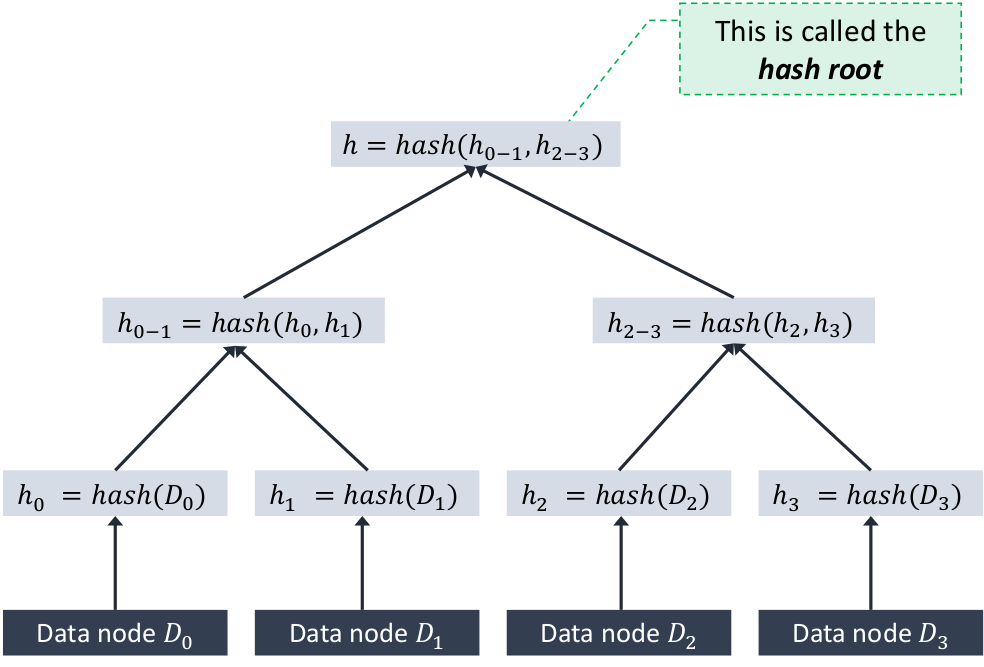
\includegraphics[width=0.8\linewidth]{figures/merkle_tree}
		\label{fig:merkletree}
	\end{subfigure}%
	\begin{subfigure}[t]{.5\textwidth}
		\centering
		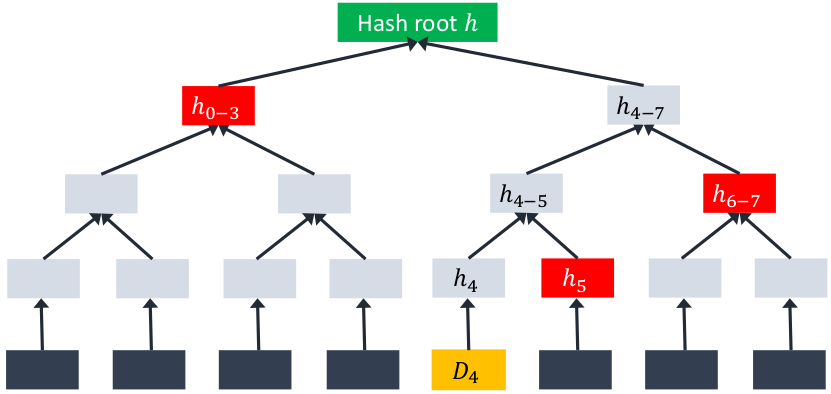
\includegraphics[width=1\linewidth]{figures/merkle_tree_verification}
		\label{fig:merkle_tree_verification}
	\end{subfigure}
\end{figure}
\vspace{-\topsep}

Data integrity verification: The \textbf{hash root $h$} is typically obtained from a trusted source. One can verify the integrity of the data elements $D_0, D_1, D_2, D_3$ by reconstructing the hash root and comparing it to the trusted root.\\

\textbf{Verifying whether $D_4$ is a member (i.e., a leaf):} Obtain the hash root $h$ from a trusted source. Then request the nodes $h_5, h_{6-7}, h_{0-3}$ (from possibly untrusted source). Finally, compute $h_4, h_{4-5}, h_{0-3}, h'$ and check whether $h = h'$.

Membership verification requires $\log(n)$ elements, only \textit{one} of which needs to be from a trusted resource (the hash root h). This is especially useful when the set of data elements is large.\\
Possible application: check if blockchain transaction is valid (i.e. in the tree).

\subsubsection{Digital signatures}

The goal of a digital signature is to allow only one user to sign but anyone to verify the signature. We have the following API for signatures:

\begin{compactitem}
	\item $(sk,pk) = generateKeys(keySize)$
	\begin{compactitem}
		\item $sk$ is the secret key, which the owner needs to keep private
		\item $pk$ is the public key, which is distributed to all users
	\end{compactitem}
	\item $sig = sign(sk, msg)$
	\item $verify(pk, msg, sig)$
\end{compactitem}

\textbf{Establish an identity:}

\begin{compactitem}
	\item User generates $(sk,pk)$ key pair
	\item $hash(pk)$ is the public name of the user
	\item $sk$ allows the user to endorse a statement $stmt$ using a digital signature $sig = sign(sk, smt)$
	\item anyone can verify statements endorsed by the user using $verify(pk, stmt, sig)$
\end{compactitem}

\subsection{Bitcoin}

In a traditional financial system, we have a centralized ledger that keeps track of everyone's balance (i.e. the amount of money). This would essentially be a very big table. In cryptocurrencies such as Bitcoin, we have a \textit{distributed ledger}. In a distributed ledger, we don't have a central table with all balances. There are multiple balances in the network. However, all nodes need to agree on the state of the ledger. For this, the ledgers run a distributed consensus protocol. Distributed consensus needs to fulfill:

\begin{compactitem}
	\item Termination: Every correct process decides on some value
	\item Agreement: All correct processes decide on the same value
	\item Validity: If all correct processes propose the same value, then any correct process must decide on that value
\end{compactitem}

Traditional motivation: reliability in distributed systems (node replication).\\

To make a transaction, users broadcast transactions to the network nodes. All nodes have a sequence of all blocks of agreed transactions they have reached consensus on. Each node has a set of outstanding transactions (to be added to a block in the blockchain). Distributed consensus in necessary since all nodes need to agree on the set of accepted transactions. Otherwise, problems such as double-spending arise.


\vspace{-\topsep}
\begin{figure}[hb]
	\centering
	\begin{subfigure}[t]{.5\textwidth}
		\centering
		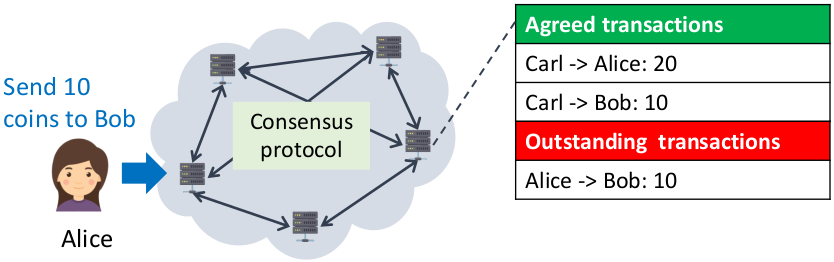
\includegraphics[width=1\linewidth]{figures/distributed_ledger_consensus}
		\label{fig:distributed_ledger_consensus}
	\end{subfigure}%
	\begin{subfigure}[t]{.5\textwidth}
		\centering
		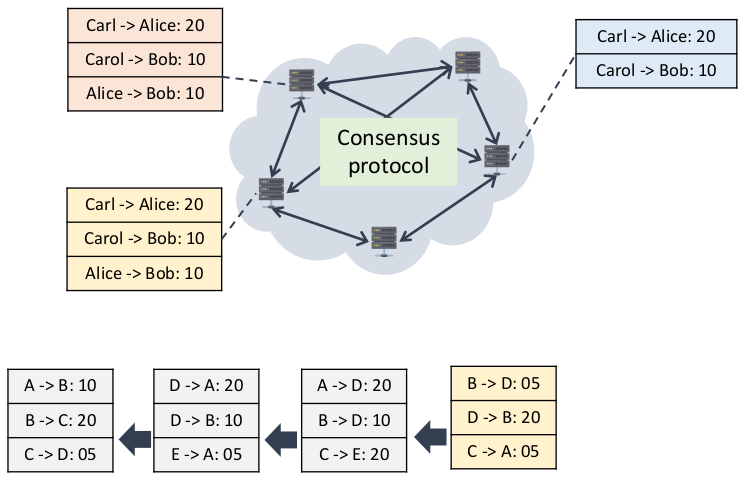
\includegraphics[width=0.6\linewidth]{figures/blockchain_overview}
		\label{fig:blockchain_overview}
	\end{subfigure}
\end{figure}
\vspace{-\topsep}

The blockchain itself as a datastrucure is essentially a linked list of blocks. A block contains a set of accepted transactions. More precisely, a block contains:

\begin{compactitem}
	\item Prev hash root: Merkle hash root of the last block
	\item Hash root $h$: Merkle hash root of the current block. The Merkle hash tree contains all transactions included in the current block. The Merkle tree enables record integrity of all transaction and efficient membership verification.
	\item Timestamp
	\item Nonce
\end{compactitem}

\begin{figure}[t!]
	\centering
	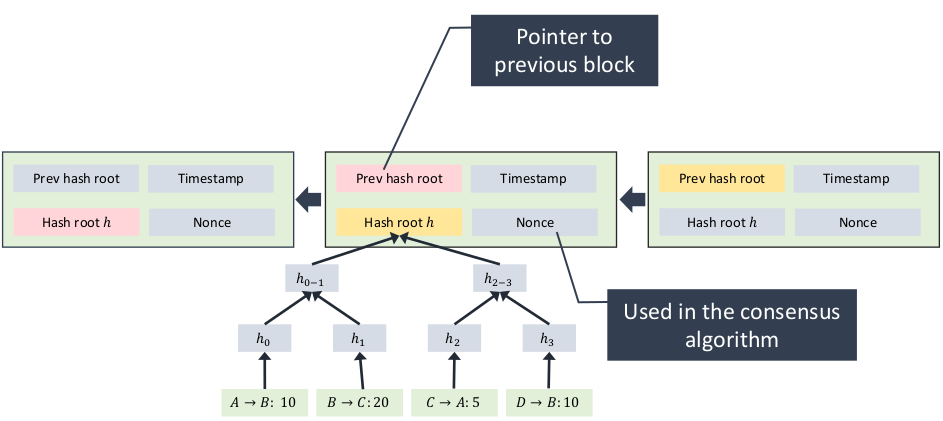
\includegraphics[width=0.6\linewidth]{figures/bitcoin_blocks}
	\label{fig:bitcoinblocks}
\end{figure}

Distributed consensus is hard: nodes may crash, nodes may be byzantine, network is imperfect (not all pairs of nodes are connected, messages may have arbitrary delays, no global time).\\

\subsubsection{Consensus algorithm (simplified)}

\begin{compactenum}
	\item New transactions are broadcast to all nodes
	\item Each node collects new transactions into a block
	\item In each round, a \textbf{random node} gets to broadcast its block
	\item Other nodes accept the block only if all transactions in it are valid (unspent, valid signatures)
	\item Nodes express their acceptance of the block by including its hash in the next block they create\\
\end{compactenum}

The question is how to select a random node. This selection needs to be careful since if we were to select nodes without randomness, it could be that nodes belonging to the same entity pick the transactions repeatedly which would for example allow the entity to censor transactions. Several schemes exist on how to pick a node: proof-of-work (select in proportion to computing power), proof-of-stake (select in proportion to ownership),... 

\subsubsection{Proof of work in Bitcoin}

Nodes need to solve a hard puzzle. Nodes have the previous block with its hash root $h_{prev}$ and the Merkle tree of the current block (with root $h$), consisting of all new transactions. The nodes then need to find a nonce $X$ such that:
$$hash(h_{prev}|h|X) \leq difficulty$$

Changing the parameter $difficulty$ adjusts the expected time it takes until a node finds a nonce $X$ (i.e. lower $difficulty$ means it takes longer). The current difficulty of Bitcoin is 15,546,745,765,529, which results in a average rate of 10.2min per block. The current hash power is 103,559,611,798 GH/s.\\
Proof-of-work makes it easy to verify: other nodes verify $hash(h_{prev}|h_{tx}) \leq difficulty$.

Key security assumption: Attacks are infeasible if majority of miners weighted by hash power follow the protocol.

\subsubsection{Double spending}

If the same output is spent in two different transactions, we have a double-spending. This results in a fork of the blockchain. Honest nodes always extend the longest valid branch. Over time, shorter branches will be abandoned. There are incentives for nodes to act honest and extend the longest chain:

\begin{compactitem}
	\item Block reward: The creator of a block can include a special coin-creation transaction in the block which will send a fixed amount of bitcoin (halfed every 210'000 blocks, currently 12.5BTC) to an chosen recipient address of this transaction. Block creator ”receives” the reward only if the block ends up on the long-term consensus branch.
	\item Transaction fees: Creator of transaction may choose to make output value less than input
	value: $\sum inputs \geq \sum outputs$. Remainder ($\sum inputs - \sum outputs$) is transaction fee that goes to the block creator.\\
	By increasing the transaction fees, you can control how fast your transaction is processed (a higher transaction fee gives a bigger incentive for miners to include the transaction in the block).\\
\end{compactitem}

Each transaction output is in one of two possible states: spent or unspent. The sum of all unspent transaction outputs (UTXOs) builds part of the shared state of the blockchain.

\subsubsection{Bitcoin scripting}

A transaction can contain a special script. 
On the most basic level, we have an unlocking script: this controls who can spend an unspent transaction output, which gives ownership. The sender uses the recipient's public key as parameter for \texttt{CHECKSIG}. The recipient then provides a signature generated with its private key (which can only be done by the holder of the private key), which is then checked by \texttt{CHECKSIG}.\\
Common Bitcoin scripts include: P2PK (Payment to public key), P2PKH (Payment to public key hash), P2MS (Pay to multi-signatures) (need multiple keys to unlock).\\

There also exists a stronger version of Bitcoin scripts: BitML - a language for Bitcoin smart
contracts. A possible application is a timed commitment:

\begin{compactitem}
	\item Alice wants to commit to a secret $s$, but reveal it sometime later.
	\item Bob wants to be assured that he will either: learn Alice's secret s within time $t$ or be compensated after time $t$.
	\item To achieve this, Alice can chooes and broadcasts $h = H(S)$ and releases two transactions:
	\begin{compactitem}
		\item (reveal h. withdraw A): Alice can reveal $s$ and spend the coin herself (i.e. send back to herself)
		\item (after t: withdraw B): Bob can spend the coin after time $t$
	\end{compactitem}
\end{compactitem}

Bitcoin scripts are limited though: no loops, no signature verification on arbitrary messages, no multiplication and shifting, no arithmetic on long numbers, no concatenation on bitstrings. Bitcoin scripting is not Turing complete.


\subsection{Smart contracts}

\begin{center}
	A smart contract formalizes the terms of a contract in code.
\end{center}

A smart contract is a \textbf{computerized transaction protocol} that executes the \textbf{terms of a contract}. The general objectives are to satisfy common contractual conditions (such as payment terms, liens, confidentiality, and even enforcement), minimize exceptions both malicious and accidental, and \textbf{minimize the need for trusted intermediaries}. Related economic goals include lowering fraud loss, arbitrations and enforcement costs, and other transaction costs.\\

\begin{center}
	\begin{tabular}{|c|c|c|}
		\hline
		& Traditional & Smart \\
		\hline
		Specification & Natural language & Code \\
		\hline
		Identity \& consent & Signatures & Digital signatures \\
		\hline
		Dispute resolution & Judges, arbitrators & Decentralized platform \\
		\hline
		Nullification & By judges & ??? \\
		\hline
		Payment & As specified & built-in \\
		\hline
		Escrow & Trusted third party & built-in \\
		\hline
	\end{tabular}
\end{center}

\subsubsection{Ethereum}

A decentralized platform designed to run smart contracts:

\begin{compactitem}
	\item Similar to a world computer that executes code and maintains the state of all smart contracts
	\item The latest block stores the latest local states of all smart contracts
	\item Transactions result in executing code (calling a function) in target smart contracts
	\item Transaction change the state of one more more contracts
	\item Ethereum smart contracts are Turing-complete
\end{compactitem}

\titlespacing{\subsection}{0pt}{2ex}{2ex}

\label{lastpage} % this must stay here
\clearpage
\addcontentsline{toc}{section}{References}
\bibliographystyle{acm}
\bibliography{refs}

\clearpage
\appendix
\pagenumbering{Roman}

\end{document}
